%% The basic ESPResSo tutorial
%%
% Writer's guide lines:
% - provide background information and references
% - do not get lost in details but maintain a nice readability
% - describe every line of the script, that contains an ESPResSo
%   command (in future tutorial, only describe new ones)
%
%%%%%%%%%%%%%%%%%%%%%%%%%%%%%%%%%%%%%%%%%%%%%%%%%%%%%%%%%%%%%%%%%
%%%%%%%%%%%%%%%%%%%%%%%%%%%%%%%%%%%%%%%%%%%%%%%%%%%%%%%%%%%%%%%%%
% From the brainstorming:
%
% Preknowledge:
%
% Basic MD(simple integrator,langevin thermostat, ---basic tcl
% basic potentials, basis tutorial 1
%
% Basis Tutorial: written in Latex
%
% <<every line of script code should be explained>>
%
% 1) tcl basic setting up a system
% MD, soft sphere and Lennard-Jones Fluid (argon system),
% Units
%
% online visualization (pdb output)
% rdf, pressure,energy,
%
% online analysis function
% savin, readin writeout, offline analysis, statistics
%
% Structure:
% Part1:
% 1) Prerequisits (what you should know beforehand: basic tcl knowledge,
% Here you can find more info: Allen, Tildesley: Frenkel smit,
% Rappaport, tcl tutorial,
%
% 2) Physics of the systems (argon, soft sphere system)
%
% 3) Algorithms (verlocity verlet, Langevin, Potentials, LJ)
% 3b) about units
%
% Part2
% 1) simulation script in all detail, line by line
% Initialize
% Visualize
% Simulate (with online analysis, saves for later off-line analysis,
% (Savelize (save our lives ))
%
% 2) a new script for later
% analysis, and other helper ideas
%
% Things to remember and take care of:
% Use the same names for variables
%
% ====================================================================
% General Tutorial: (the next tutorials: pe_solution, cell model of one
% charged colloid, LB, ferrofluid)
%

% basiert auf KOMA-Script scrbook-Klasse
\documentclass[11pt,a4paper,% BCOR8mm,
	       %twoside, onecolumn, openright, cleardoubleempty, %
	       %parindent,
headnosepline, footnosepline, notitlepage, %
	       %onelinecaption,
bigheadings, % bibtotoc, %tocindent, listsindent, %
	       %chapterprefix, noappendixprefix,
	       %tablecaptionbelow,
	       %pointlessnumbers, % macht Probleme (Anhang ohne Punkt, aber sonst Kapitel mit Punkt
	       % abstractoff, fleqn, leqno,
	       % openbib, origlongtable,
final]{scrartcl}

% Satzspiegel

% wenn keine KOMA-Klasse verwendet wird, kann so der Satzspiegel
% berechnet werden
%\usepackage[DIV15,BCOR12mm,pagesize]{typearea}

% Hier knnen Seitenhoehe und -breite individuell angepasst werden
%\areaset[BCOR]{Breite}{Hohe}
% oder
%\usepackage[a4paper,body={15.6cm,23cm},left=3cm]{geometry}

% ============================================================================

%% Grafikpakete
% Fr einfache Einbingung von Grafiken
\usepackage{graphicx}%
\usepackage{framed, color}

% Wenn man direkt mit dem pdflatex eine PDF-Datei erzeugt, sollten diese beiden
% Pakete eingebunden werden (Hyperlinks, bessere Bildschirmschriftarten usw.)
\usepackage{color}
\definecolor{mylinkcolor}{rgb}{0.5812,0.0665,0.0659} % IndianRed
\definecolor{mycitecolor}{rgb}{0.075,0.31,0.0431} % MossGreen
\definecolor{myurlcolor}{rgb}{0.0118,0.098,0.7412} % DarkBlue
\usepackage[pdftex,bookmarks]{hyperref}

% Druckversion
% f�r reine pdf-Dateien noch Option colorlinks hinzufgen, um Links farbig zumachen
% \usepackage[pdftex,bookmarks,bookmarksopen,citecolor={mycitecolor},%
%  linkcolor={mylinkcolor},urlcolor={myurlcolor},breaklinks=true,%
%  hypertexnames=false,hyperindex=true,encap,colorlinks]{hyperref} %

%  	\hypersetup{
%     pdftitle = {},
%     pdfauthor = {Kai Grass},
%     pdfsubject = {},
%     pdfkeywords = {},
%     pdfcreator = {},%
%     pdfproducer = {},
% 	}%

\usepackage{ae,aecompl}

% ============================================================================

%% Sprachliche Pakete
\usepackage[english]{babel}
% Neue Deutsche Rechtschreibung
%\usepackage[ngerman]{babel}
%\usepackage{ngerman}

% Paket zur einfacheren Eingabe deutscher Umlaute
%\usepackage[applemac]{inputenc} %Mac
\usepackage[latin1]{inputenc}   %UNIX/LINUX
% \usepackage[ansinew]{inputenc}  % Windows
%\usepackage[T1]{fontenc}

% ============================================================================

% Literaturverzeichnis
\usepackage[square,numbers,sort&compress]{natbib}
%\usepackage{bibmods}
%\bibpunct{(}{)}{,}{a}{}{,}
%\bibpunct{(}{)}{,}{a}{,}{;}
\setlength{\bibsep}{1ex}

% ============================================================================

% Stichwortverzeichnis
% \usepackage{makeidx}
% \makeindex

% ============================================================================

% Deutsche Zahlenkonvention (1 (Komma) 0 statt 1 (Punkt) 0)
% \usepackage{ziffer}

%% Schriftarten
\usepackage{times} % times is used to avoid bitmap fonts in PDF

%% Mathematische Packages
% Dieses Pakete definiert viele ntzliche mathematische Befehele und
% Die Option "intlimits" bewirkt, dass beim Integral die Grenzenangaben oben
% und unten erscheinen und nicht seitlich.
\usepackage[intlimits]{amsmath}
\usepackage{amsfonts}
\usepackage{amsthm}
\usepackage{mathrsfs}
\usepackage{stmaryrd}


% Diese Schriftarten ermglichen schne Mengensymbole fr natrliche Zahlen, usw.
% siehe Definition von \N, \Z usw. Dies ist Geschmackssache.
%\usepackage{bbm}
%\usepackage{dsfont}

% Subfigures
\usepackage{subfigure}

% Needed for Tabular-Umgebung
\usepackage{array}

% werden (sog. Schusterjungen und Hurenkinder vermeiden)
%\clubpenalty = 10000
%\widowpenalty = 10000

\sloppy

% Ein Paket um "kommutative Diagramme" zu erstellen. Fuer einfhrende Beispiele
% siehe xymanual.ps und xyreference.ps
%\usepackage[all]{xy}

%%%%%%%%%%%%%%%%%%% Shortcuts %%%%%%%%%%%%%%%%%%%%%%%%%%%%%%%%%%%%%%%%%%%%
%\newcommand{\N}{\mathbbm{N}}	% Natuerliche Zahlen
%\newcommand{\Z}{\mathbbm{Z}}	% Ganze Zahlen
%\newcommand{\Q}{\mathbbm{Q}}	% Rationale Zahlen
%\newcommand{\R}{\mathbbm{R}}	% Reelle Zahlen
%\newcommand{\C}{\mathbbm{C}}	% Komplexe Zahlen
%\newcommand{\one}{\mathbbm{1}}	% Einheits Eins
%
%\newcommand{\toinf}{\to\infty}				% --> oo
%\newcommand{\tozero}{\to 0}				% --> 0
%\newcommand{\ontop}[2]{\genfrac{}{}{0pt}{}{#1}{#2}}	% Aufeinander
%\newcommand{\abs}[1]{\left|#1\right|}
%\newcommand{\argmax}{\mathop{\rm arg\,max}}

% Ein Befehl, um Abbildungen einfach einheitlich zu gestalten
% Bsp: \abb{f}{\R}{\R}{x}{x^2}

%\newcommand{\abb}[5]{%
%\setlength{\arraycolsep}{0.4ex}%
%\begin{array}{rcccc}%
%#1 &:\,& #2 & \,\,\longrightarrow\,\, & #3 \\[0.5ex]%
%     & & #4 & \longmapsto & #5%
%\end{array}%
%}

%%%%%%%%%%%%%%%%%%% Theorem definitions %%%%%%%%%%%%%%%%%%%%%%%%%%%%%%%%%%
%\theoremstyle{plain}
%\newtheorem{theorem}{Theorem}[chapter]
%\newtheorem{proposition}[theorem]{Proposition}
%\newtheorem{lemma}[theorem]{Lemma}
%\newtheorem{satz}[theorem]{Satz}
%\newtheorem{korollar}[theorem]{Korollar}
%
%\theoremstyle{definition}
%\newtheorem{definition}{Definition}[chapter]
%\newtheorem{beispiel}[theorem]{Beispiel}
%\newtheorem{bemerkung}[theorem]{Bemerkung}
%
%%%%%%%%%%%%%%%%%%%%%%%%%%%%%%%%%%%%%%%%%%%%%%%%%%%%%%%%%%%%%%%%%%%%%%%%%%

% ============================================================================
% \renewcommand*{\partpagestyle}{empty}
% \renewcommand*{\partformat}{\partname~\thepart:}
%\usepackage{fancyhdr}
%%\pagestyle{headings}
%\pagestyle{fancyplain}
%%\addtolength{\headwidth}{\marginparsep}
%%\addtolength{\headwidth}{\marginparwidth}
%\renewcommand{\chaptermark}[1]{\markboth{#1}{}}
%\renewcommand{\sectionmark}[1]{\markright{\thesection\ #1}}
%%\lhead[\fancyplain{}{\bfseries\thepage}]{\fancyplain{}{\bfseries\rightmark}}
%\lhead[\fancyplain{}{\thepage}]{\fancyplain{}{\rightmark}}
%%\rhead[\fancyplain{}{\bfseries\leftmark}]{\fancyplain{}{\bfseries\thepage}}
%\rhead[\fancyplain{}{\leftmark}]{\fancyplain{}{\thepage}}
%%\chead{}
%%\rhead{\thepage}
%%\lfoot{Schnellste Pfade in geometrischen Netzwerken}
%\cfoot{}
%%\rfoot{}
%%\setlength{\headrulewidth}{0.4pt}
%%\setlength{\footrulewidth}{0.4pt}

%\usepackage[automark]{scrpage2}
%\pagestyle{scrheadings}
%\automark[section){chapter}
%\lehead[scrplain-links-gerade]{scrheadings-links-gerade}
%\cehead[scrplain-mittig-gerade]{scrheadings-mittig-gerade}
%\rehead[scrplain-rechts-gerade]{scrheadings-rechts-gerade}
%\lefoot[scrplain-links-gerade]{scrheadings-links-gerade}
%\cefoot[scrplain-mittig-gerade]{scrheadings-mittig-gerade}
%\refoot[scrplain-rechts-gerade]{scrheadings-rechts-gerade}
%\lohead[scrplain-links-ungerade]{scrheadings-links-ungerade}
%\cohead[scrplain-mittig-ungerade]{scrheadings-mittig-ungerade}
%\rohead[scrplain-rechts-ungerade]{scrheadings-rechts-ungerade}
%\lofoot[scrplain-links-ungerade]{scrheadings-links-ungerade}
%\cofoot[scrplain-mittig-ungerade]{scrheadings-mittig-ungerade}
%\rofoot[scrplain-rechts-ungerade]{scrheadings-rechts-ungerade}
%\ihead[scrplain-innen]{scrheadings-innen}
%\chead[scrplain-zentriert]{scrheadings-zentriert}
%\ifoot[scrplain-innen]{scrheadings-innen}
%\cfoot[scrplain-zentriert]{scrheadings-zentriert}
% Markierungen: \leftmark, \rightmark, \pagemark \headmark
% \manualmark \automark

% ============================================================================

%%%%%%%%%%%%%%%%%%%%%%%%%%%%%%%%%%%%%%%%%%%%%%%%%%%%%%%%%%%%%%%%%%%%%%%%%%
\setcounter{secnumdepth}{2}
\setcounter{tocdepth}{1}
%%%%%%%%%%%%%%%%%%%%%%%%%%%%%%%%%%%%%%%%%%%%%%%%%%%%%%%%%%%%%%%%%%%%%%%%%%

%% Schriftsatz in KOMA
%\setkomafont{Element}{Befehle}
%\addtokomafont{Element}{Befehle}
%\usekomafont{Element}

%\includeonly{kapitel/sinterkeramiken, kapitel/statisch, kapitel/dynamisch, kapitel/ergebnisse, kapitel/abbildungen,
% kapitel/literatur}
%\includeonly{kapitel/titelseite2}
% ============================================================================

\usepackage{verbatim}

% \usepackage[usenames,dvipsnames]{xcolor}
% \definecolor{codebg}{rgb}{0.95,0.95,0.95}
% \definecolor{codeframe}{gray}{0.5}
% \definecolor{codeshadow}{gray}{0.7}
% \definecolor{codenumber}{rgb}{0.58,0,0.82}
% \definecolor{pblau}{rgb}{0.09375,0.19921875,0.4296875}


% \usepackage{listings}
% \lstset{
%   basicstyle=\ttfamily,
% 	keywordstyle=\bfseries\ttfamily\color[rgb]{0.65,0.16,0.18},
% 	identifierstyle=\ttfamily\color{black},
% 	commentstyle=\color{pblau},
% 	stringstyle=\ttfamily\color[rgb]{0.627,0.126,0.941},
% 	showstringspaces=false,
% 	tabsize=2,
% 	breaklines=true,
% 	prebreak = \raisebox{0ex}[0ex][0ex]{\ensuremath{\hookleftarrow}},
% 	breakatwhitespace=false,
% 	numberstyle=\footnotesize \normalfont \sffamily,
% 	numbers=left,
% 	stepnumber=1,
% 	numbersep=1.5em,
%   xleftmargin=2.7em,
%   framexleftmargin=2.7em,
% 	aboveskip={1\baselineskip},
% 	belowskip={1\baselineskip},
%   columns=fixed,
%   upquote=true,
%   extendedchars=true,
%   frame=shadowbox,
%   rulesepcolor=\color{codeshadow},
%   rulecolor=\color{codeframe},
%   backgroundcolor=\color{codebg},
%   mathescape=false,
%   language=python
% }


% The ESPResSo Logo
% how to define it such that there is a space afterwards if needed
% but not, when there is a point afterwards ????
\newcommand{\ES}{\textbf{ESPResSo}}

% How to diplay ESPResSo commands in flowing text. Larger code segments
% should be put inside boxes.
\newcommand{\EScmd}[1]{\texttt{\textbf{#1}}}

% The code block
%\newcommand{\EScode}[1]{ \parbox{0.95\textwidth}{\texttt{#1}}}
%\usepackage{listings}
%\lstset{numbers=left, numberstyle=\tiny, numbersep=5pt, showspaces=false, showstringspaces=false,postbreak=\space, breakindent=5pt, breaklines}
%\lstset{language=tcl, keywordstyle=\color{blue}\bfseries ,emphstyle=\color{green}, commentstyle=\color{red}\itshape }
%\lstset{keywordsprefix=setmd}
%\lstset{keywords=[6]{thermostat,part,inter,integrate,rescale_velocities,save_sim,writepdb,analyze, lbnode, lb_boundary, lbfluid, constraint}}

% Copyright (C) 2010,2011,2012,2013,2014,2015,2016 The ESPResSo project
% Copyright (C) 2002,2003,2004,2005,2006,2007,2008,2009,2010
%  Max-Planck-Institute for Polymer Research, Theory Group
%  
% This file is part of ESPResSo.
%   
% ESPResSo is free software: you can redistribute it and/or modify it
% under the terms of the GNU General Public License as published by the
% Free Software Foundation, either version 3 of the License, or (at your
% option) any later version.
%  
% ESPResSo is distributed in the hope that it will be useful, but
% WITHOUT ANY WARRANTY; without even the implied warranty of
% MERCHANTABILITY or FITNESS FOR A PARTICULAR PURPOSE.  See the GNU
% General Public License for more details.
%  
% You should have received a copy of the GNU General Public License
% along with this program.  If not, see <http://www.gnu.org/licenses/>.
%
\usepackage[draft]{varioref}    % defines \vref
\usepackage{hyperref}           % automatically creates links when
                                % using pdflatex, defines \url
\usepackage{ifpdf}              % defines \ifpdf
\usepackage{graphicx}           % handles graphics
\usepackage{color}              % use colors

\usepackage{amsmath}

\usepackage{verbatim}           % required for \verbatim and \endverbatim
\usepackage{fancyvrb}
\usepackage{calc}               % compute length
\usepackage{ifthen}             % provide ifthen
\usepackage{xspace}
\usepackage{units}
\usepackage[numbers]{natbib}

\usepackage{listings}

% For building the distribution docs, disable todo boxes.
%\usepackage[disable]{todonotes}
\usepackage{todonotes}

\newcommand{\es}{\mbox{\textsf{ESPResSo}}\xspace}
\newcommand{\ie}{\textit{i.e.}\xspace}
\newcommand{\eg}{\textit{e.g.}\xspace}
\newcommand{\etal}{\textit{et al.}\xspace}

\newcommand{\codebox}[1]%
{\texttt{#1}}

\DefineVerbatimEnvironment{code}{Verbatim}%
{commandchars=\\\{\}}
\makeatletter
\newenvironment{tclcode}
{%
  \addtolength{\linewidth}{-2em}% set the line length
  \@minipagetrue%%%DPC%%%
  \@tempswatrue%%%DPC%%%
  \hsize=\linewidth%
  \setbox0=\vbox\bgroup\verbatim
}{\endverbatim
  \unskip\setbox0=\lastbox%%%DPC%%%
  \egroup
  \par%
  \noindent\hspace{1em}%
  \codebox{\box0}%
  \par\noindent%
}
\makeatother

% \newcommand{\todo}[1]{
%   \marginpar{%
%     \setlength{\fboxrule}{1pt}
%     \fcolorbox{red}{yellow}{%
%       \parbox{\marginparwidth-2\fboxrule-2\fboxsep}{%
%         \bf\raggedright\scriptsize #1%
%       }%
%     }%
%   }%
% }

\makeatletter
\renewcommand{\minisec}[1]{\@afterindentfalse \vskip 1.5ex
  {\parindent \z@
    \raggedsection\normalfont\sffamily\itshape\nobreak#1\par\nobreak}%
  \@afterheading}
\makeatother

\newcommand{\esptitlehead}{
  \titlehead{
    \begin{center}
      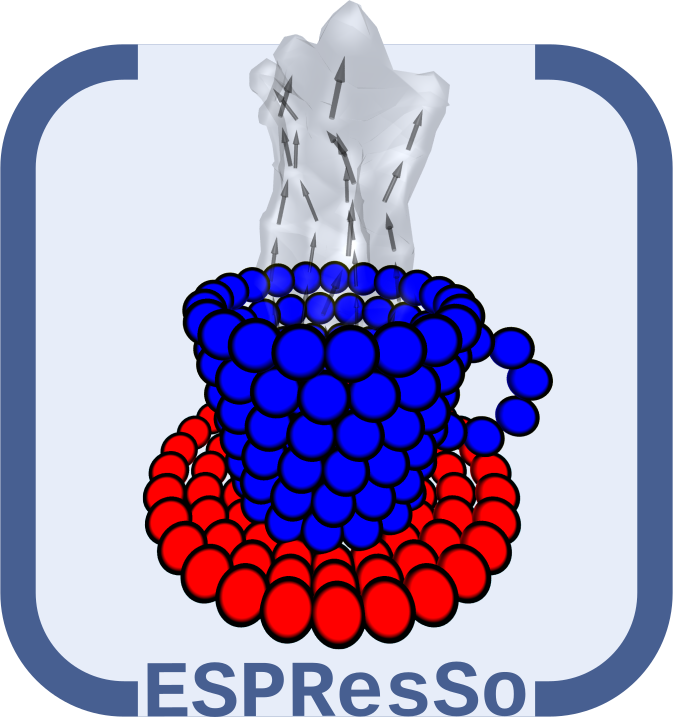
\includegraphics[width=5cm]{logo/logo.pdf}
    \end{center}
  }
}

% Do magic that \bfseries for keywords actually works
\DeclareFontShape{OT1}{cmtt}{bx}{n}{<5><6><7><8><9><10><10.95><12><14.4><17.28><20.74><24.88>cmttb10}{}

% Custom colors
\definecolor{stringblue}{rgb}{0.09,0.211,0.57}
\definecolor{codered}{rgb}{0.655,0.1137,0.3747}
\definecolor{deepgreen}{rgb}{0,0.5,0}
\definecolor{commentgray}{rgb}{0.4,0.4,0.4}
\definecolor{framegray}{rgb}{0.8,0.8,0.8}

% Python style for highlighting
\newcommand\pythonstyle{\lstset{
    language=Python,
    belowskip=\bigskipamount,
    aboveskip=\bigskipamount,
    basicstyle=\ttfamily\small,
    otherkeywords={self},             % Add keywords here
    keywordstyle=\bfseries\color{codered},
    emph={MyClass,__init__},          % Custom highlighting
    emphstyle=\bfseries\color{deepgreen},    % Custom highlighting style
    commentstyle=\color{commentgray}\ttfamily,
    stringstyle=\color{stringblue},
    frame=tb,                         % Any extra options here
    rulecolor=\color{framegray},
    showstringspaces=false            % 
    }
}


% Python environment
\lstnewenvironment{python}[1][]{\pythonstyle \lstset{#1}}{}

% Python for external files
\newcommand\pythonexternal[2][]{{\pythonstyle \lstinputlisting[#1]{#2}}}

% Python for inline
\newcommand\pythoninline[1]{{\pythonstyle\lstinline!#1!}}



\newtheorem{task}{Task}

\begin{document}
\renewcommand{\d}{\mathrm d}
\subject{ESPResSo Tutorial}
\title{The GPU Electrokinetics Method in \ES{}:
Electroosmotic Flow
} %\author{ Georg Rempfer \thanks{\ttfamily georg@icp.uni-stuttgart.de}}
\date{\today}
\publishers{Institute for Computational Physics, University of Stuttgart}
\maketitle 
\begin{center}
  \includegraphics[width=0.7\columnwidth]{figures/schlitzpore_3d.pdf}
\end{center}
\pagebreak
\definecolor{mygray}{gray}{.75}
%\begin{center}
%  \colorbox{mygray}{ 
%\begin{minipage}[h]{13cm}
%  {\bf \large Before you start:}\\
%  With this tutorial you can get started using the Electrokinetics method
%  for scientific applications. We give a brief introduction about the theory
%  and how to use it \ES{}. 
%  We have selected one sample problem for which an analytic solution exists.
%\end{minipage}
%}
%\end{center}

 \tableofcontents
 \pagebreak
  
\section{Introduction}

%\floatingBox{5}{4cm}{Mein Text der in der Box abgebildet werden soll. Mal schauen wie das klappt.} 

In recent years the lattice-Boltzmann method (LBM) has proven itself to be a viable way to introduce hydrodynamic interactions into coarse-grained MD simulations with moderate computational cost. The success of the GPU LBM implementation in \ES{} and similar developments in other software packages created demand for further developments in this area. \ES{} features two such algorithms, namely ELECTROHYDRODYNAMICS, and ELECTROKINETICS (EK). Both of these make use of the LBM and extend it to coarse-grain not only the solvent molecules but also ionic solutes. ELECTROHYDRODYNAMICS does so using a slip layer coupling for charged particles valid in the thin Debye layer (large salt concentration) limit\cite{hickey10a}, while EK explicitly treats the ionic solutes in a continuum fashion and is valid for a wide range of salt concentrations\cite{capuani04a,rempfer13a,rempfer16a}.

\subsection*{Tutorial Outline}

To make our first steps using ELECTROKINETICS we will work on one of the few systems for which analytic solutions for the electrokinetic equations exist -- the slip pore geometry with a counterion-only electrolyte. The same slit pore system is also treated in the LBM tutorial, but there, the ionic species were modeled as explicit particles. For this system, the two approaches lead to exactly the same results~\cite{rempfer10a}. Differences are only becoming significant for multivalent ions, very high salt concentrations, and very high surface charge, since then the mean-field approach the EK is employing, basically solving the Poisson-Nernst-Planck formalism plus the Navier-Stokes equation on a lattice, gives significantly different results from explicit ion approaches \cite{deserno00a,holm01a,deserno01c}.

This tutorial is divided into three sections. The first section~\ref{sec:theory} introduces the electrokinetic equations and the analytical solution for the slit pore system, while the second section~\ref{sec:simulation} deals exclusively with the simulation, its setup, and the results.

If you already know about simple diffusion-migration-advection equations, continuum electrostatics, and Navier-Stokes, then you can skip the first section.

\pagebreak

% Copyright (C) 2010,2011 The ESPResSo project
%  
% This file is part of ESPResSo.
%   
% ESPResSo is free software: you can redistribute it and/or modify it
% under the terms of the GNU General Public License as published by the
% Free Software Foundation, either version 3 of the License, or (at your
% option) any later version.
%  
% ESPResSo is distributed in the hope that it will be useful, but
% WITHOUT ANY WARRANTY; without even the implied warranty of
% MERCHANTABILITY or FITNESS FOR A PARTICULAR PURPOSE.  See the GNU
% General Public License for more details.
%  
% You should have received a copy of the GNU General Public License
% along with this program.  If not, see <http://www.gnu.org/licenses/>.
%

\chapter{Lattice-Boltzmann}
\label{sec:lb}
\newescommand{lb}

For an implicit treatment of a solvent, \es allows to couple the
molecular dynamics simulation to a Lattice-Boltzmann fluid. The Lattice-
Boltzmann-Method (LBM) is a fast, lattice based method that allows in its
``pure'' form to calculate fluid flow in different boundary conditions
also in complex geometries. Coupled to molecular dynamics, it allows
to take hydrodynamic interactions into account
computationally efficiently. The implementation of boundary conditions
for the LBM is a difficult task, where still a lot of research is going 
on. The focus of the \es implementation of the LBM is, of course, the
coupling to MD and therefore available geometries and boundary
conditions are somewhat limited compared to ``pure'' codes. 


Here we restrict the documentation on the interface. For a more detailed
description of the method, please refer to the literature.

\section{Setting up and LB fluid}
\begin{essyntax}
  lbfluid
  \opt{agrid  \var{agrid}}
  \opt{dens  \var{density}}
  \opt{visc  \var{viscosity}}
  \opt{tau  \var{lb\_timestep}}
  \opt{bulk_visc  \var{bulk\_viscosity}}
  \opt{ext_force  \var{f_x} \var{f_y} \var{f_z}}
  \opt{friction   \var{gamma} } 
  \opt{gamma_odd  \var{gamma\_odd}}
  \opt{gamma_even  \var{gamma\_even}}
  \begin{features}
  \required{LB}
  \end{features}
\end{essyntax}
The \lit{lbfluid} command initializes the fluid with a given
set of parameters. It is also possible to change parameters on the
fly, but this will only rarely be done in practice. Before being able
to use the LBM, it is necessary to set up a box of a desired size. The
parameter \lit{agrid} is used to set the lattice constant of the
fluid, so the size of the box in every direction must be a multiple of
\var{agrid}.

In \es the LB scheme and the MD scheme are not synchronized: In one LB
time step typically several MD steps are performed. This allows to
speed up the simulations and is adjusted with the parameter \var{tau},
the LB timestep.
The parameters \var{dens} and \var{visc} set up the density and
viscosity of the LB fluid in (usual) MD units.  Internally the LB
implementation works with a different set of units: all lengths are
expressed in \var{agrid}, all times in \var{tau} and so on.  Therefore
changing \var{agrid} and \var{tau}, might change the behaviour of the
LB fluid, \eg at boundaries, due to characteristics of the LBM
itself. Currently it is not possible to precisely give a parameter set
where reliable results are expected, but we are currently performing a
study on that. Therefore the LBM should \emph{not be used as a black
  box}, but only after a careful check of all parameters that were
applied. 

The parameter \lit{ext_force} allows to apply an external body force
density that is homogeneous over the fluid. It is again to be given in
MD units.  The parameter \lit{bulk_viscosity} allows to tune the bulk
viscosity of the fluid and is given in MD units. In the limit of low
Mach (often also low Reynolds) number the results should be
independent of the bulk viscosity up to a scaling factor. 
It is however known that the values of the viscosity does 
affect the quality of the implemented link-bounce-back method.
\lit{gamma_odd} and
\lit{gamma_even} are the relaxation parameters for the kinetic
modes. Due to their somewhat obscure nature they are to be given
directly in LB units.

Before running a simulation at least the following parameters must be
set up: \lit{agrid}, \lit {dens}, \lit{visc}, \lit{tau},
\lit{friction}. For the other parameters, the following are taken:
\var{bulk\_viscosity}=0, , \var{gamma\_odd}=0, \var{gamma\_even}=0,
\var{ f_x} = \var{ f_y} = \var{ f_z} = 0.

\section{LB as a thermostat}
\begin{essyntax}
  thermostat lb \var{T} 
  \begin{features}
  \required{LB}
  \end{features}
\end{essyntax}
The LBM implementation in \es uses Duenweg's point coupling method
to couple MD particles the LB fluid. This coupling consists
in a frictional force and a random force:
\begin{equation*}
  \vec{F} = -\gamma \left(\vec{v}-\vec{u}\right) + \vec{F}_R.
\end{equation*}
The frictional force tends to decrease the relative velocity
between the fluid and the particle whereas the random forces are chosen
so large that the average kinetic energy per particle corresponds to
the given temperature, according to a fluctuation dissipation theorem.
No other thermostatting mechanism is necessary then. Please any of these
off before starting the LB thermostatting mechanism.

The LBM implementation provides a fully thermalized LB fluid, \ie all
nonconserved modes, including the pressure tensor, fluctuate correctly
according to the given temperature and the relaxation parameters. All
fluctuations can be switched off by setting the temperature to 0.


\section{Reading and setting single lattice nodes}
\begin{essyntax}
  lbnode \var{x} \var{y} \var{z} \alt{print \asep set} \var{args}
  \begin{features}
  \required{LB}
  \end{features}
\end{essyntax}
The \lit{lbnode} command allows to inspect (\lit{print}) and modify
(\lit{set}) single LB nodes.  Note that the indexing in every
direction starts with 0.  For both commands you have to specify what
quantity should be printed
or modified. Print allows the following arguments: \\
\begin{tabular}{p{0.2\columnwidth}p{0.5\columnwidth}}
  \lit{rho}\ & the density (scalar). \\
  \lit{u} & the fluid velocity (three floats: $u_x$, $u_y$, $u_z$) \\
  \lit{pi} & the fluid velocity (six floats: $\Pi_{xx}$, $\Pi_{xy}$, $\Pi_{yy}$, $\Pi_{xz}$,  $\Pi_{yz}$,  $\Pi_{zz}$) \\
  \lit{pi_neq} & the nonequilbrium part of the pressure tensor, components as above. \\
  \lit{pop} & the 19 population (check the order from the source code please).
\end{tabular} \\
Example:
The line
\begin{tclcode}
puts [ lbnode 0 0 0 print u ]
\end{tclcode}
prints the fluid velocity in node 0 0 0 to the screen.  The command
\lit{set} allows to change the density or fluid velocity in a single
node. Setting the other quantities can easily be implemented.
Example:
\begin{tclcode}
puts [ lbnode 0 0 0 set u 0.01 0. 0.]
\end{tclcode}

\section{Setting up boundary conditions}
\begin{essyntax}
  lbboundary \var{shape} \var{shape\_args} 
  \begin{features}
  \required{LB_BOUNDARIES}
  \end{features}
\end{essyntax}
If nothing else is specified periodic boundary conditions are assumed 
for the LB fluid. The \lit{lbboundary} command allows to set up
other (internal or external) boundaries.

The \lit{lbboundary} command syntax is very close to the
\lit{constraint} syntax, as usually one wants the hydrodynamic
boundary conditions to be shaped similar to the MD
boundaries. Currently the above mentioned shapes are available and
their syntax follows exactly the syntax of the constraint command. For
example
\begin{tclcode}
  lbboundary wall dist 1.5 normal 1. 0. 0. 
\end{tclcode}
creates a planar boundary condition at distance 1.5 from the origin of
the coordinate system where the half space $x>1.5$ is treated as
normal LB fluid, and the other half space is filled with boundary
nodes.

Intersecting boundaries are in principle possible but must be treated
with care. In the current, only partly satisfactory, implementation for
every LB node the closest boundary is determined and in case of a
negative distance to that boundary (meaning being inside the wall)
lets \es decide that it is a wall node, and a positive one, that it is
not.  This allows example multiple parallel channels, but is is not
always clear that a rectangularly shaped channel can be
constructed. Suggestions on how to solve this issue are very welcome.

Currently, only the so called ``link-bounce-back'' algorithm for wall
nodes is available. This creates a boundary that is located
approximately midway between the lattice nodes, so in the above
example this corresponds indeed to a boundary at $x=1.5$. Note that
the location of the boundary is unfortunately not independent of the
viscosity. This can \eg be seen when using the sample script
\lit{poisseuille.tcl} with a high viscosity.

\section{Choosing between the GPU and CPU implementations}
\begin{essyntax}
  \variant{1} lbfluid cpu
  \variant{2} lbfluid gpu
  \begin{features}
    \required[1]{LB}
    \required[2]{LB_GPU}
  \end{features}
\end{essyntax}

A very recent development is an implementation of the LBM for NVIDIA
GPUs using the CUDA framework.  On CUDA-supporting machines this can
be activated by configuring with \lit{configure
  --with-cuda=/path/to/cuda} and activating the feature \lit{LB_GPU}.
Within the \es-Tcl-script, the \lit{lbfluid} command can be used to
choose between the CPU and GPU implementations of the
Lattice-Boltzmann algorithm, for further information on CUDA support
see section~\ref{sec:cuda}.

Variant \variant{1} is the default and turns on the standard CPU
implementation of the Lattice-Boltzmann fluid, while variant
\variant{2} turns on the GPU implementation, implying that all
following LB-related commands are executed on the GPU.

Currently only a subset of the CPU commands are available for the GPU
implementation.  For boundary conditions analogous to the CPU
implementation, the feature \lit{LB_BOUNDARIES_GPU} has to be
activated.

%%% Local Variables:
%%% mode: latex
%%% TeX-master: "ug"
%%% End:



\section{The LB interface in \ES{}}
\ES{} features two virtually independent implementations of LB. One implementation
uses CPUs and one uses a GPU to perform the computational work. If in the first usage
of the command { \tt lbfluid} the parameter {\tt gpu} is given as first
parameter, the GPU will be used.

The LB lattice is a cubic lattice, with a lattice constant {\tt agrid} that
is the same in all spacial directions. The chosen box length must be an integer multiple
of {\tt agrid}. The LB lattice is shifted by 0.5 {\tt agrid} in all directions: the node
with integer coordinates $\left(0,0,0\right)$ is located at
$\left(0.5a,0.5a,0.5a\right)$.
The LB scheme and the MD scheme are not synchronized: In one
LB time step typically several MD steps are performed. This allows to speed
up the simulations and is adjusted with the parameter {\tt tau}.
The LB parameter {\tt tau} must be an integer multiple of the MD timestep.

Even if MD features are not used a few MD parameters must be set, although they are irrelevant
to the LB module. These is mainly {\tt skin}, but also the MD timestep has to be
set as the command {\tt integrate} is used to propagate MD steps. LB steps are performed 
in regular intervals, such that the timestep $\tau$ for LB is recovered. 

\ES{} has three main commands for the LB module: 
 {\tt lbfluid},  {\tt lbnode}, and  {\tt lbboundary}.
 {\tt lbfluid} is mainly used to set up parameters and does everything that
concerns the whole fluid.  {\tt lbnode} involves readout and manipulation of
single LB cells.  {\tt lbboundary} allows to set boundaries, currently only
the bounce back boundary method is implemented to model
no-slip walls. Additionally the command  {\tt thermostat lb} is used to set
the temperature. 


Important Notice: All commands of the LB interface use
MD units. This is convenient, as e.g. a particular 
viscosity can be set and the LB time step can be changed without
altering the viscosity. On the other hand this is a source
of a plethora of mistakes: The LBM is only reliable in a certain 
range of parameters (in LB units) and the unit conversion
may take some of them far out of this range. So note that you always
have to assure that you are not messing with that!

One brief example: a certain velocity may be 10 in MD units.
If the LB time step is 0.1 in MD units, and the lattice constant
is 1, then it corresponds to a velocity of 1 in LB units. 
This is the maximum velocity of the discrete velocity set and therefore
causes numerical instabilities like negative populations.

\subsection*{The {\tt lbfluid} command}
The {\tt lbfluid} command sets global parameters of the LBM. Every
parameter is given in the form {\tt lbfluid name value}. 
All parameters except for {\tt gamma\_odd} and  {\tt gamma\_even}
are given in MD units. All parameters except for {\tt ext\_force} accept
one scalar floating point argument. \\
\vspace{0,2cm}
\begin{tabular}{p{0.2\columnwidth}p{0.5\columnwidth}}
{\tt dens} & The density of the fluid.\\
{\tt grid} & The lattice constant of the fluid. It is used to determine the number of LB nodes 
per direction from {\tt box\_l}. {\em They have to be compatible.} \\
{\tt visc} & The kinematic viscosity \\
{\tt tau} & The time step of LB. It has to be equal or larger than the MD time step. \\
{\tt friction} & The friction coefficient $\gamma$ for the coupling scheme. \\
{\tt ext\_force} & An external force applied to every node with three components. \\
{\tt gamma\_odd} & Relaxation parameter for the odd kinetic modes. \\
{\tt gamma\_even} & Relaxation parameter for the even kinetic modes.
\end{tabular} \\
\vspace{0,2cm}

A good starting point for an MD time step of 0.01 is the command line
\vspace{0,2cm}
\begin{lstlisting}[ numbers=none]
lbfluid grid 1.0 dens 10. visc .1 tau 0.01 friction 10.
\end{lstlisting}
\vspace{0,2cm}

\subsection*{The {\tt lbnode} command}
The {\tt lbnode} command allows to inspect and modify single LB nodes The
general syntax is:
\vspace{0,2cm}
\begin{lstlisting}[ numbers=none]
lbnode X Y Z command arguments
\end{lstlisting}
\vspace{0,2cm}
Note that the indexing in every direction starts with 0. The possible commands are:
\vspace{0,8cm}
\begin{tabular}{p{0.2\columnwidth}p{0.5\columnwidth}}
  print & Print one or several quantities to the TCL interface.\\
  set & Set one quantity to a particular value (can be a vector)\\
\end{tabular}\\
\vspace{0,8cm}
For both commands you have to specify what quantity should be printed
or modified. Print allows the following arguments: \\


\vspace{0,8cm}
\begin{tabular}{p{0.2\columnwidth}p{0.5\columnwidth}}
  {\tt rho}\ & the density (scalar). \\
  {\tt u} & the fluid velocity (three floats: $u_x$, $u_y$, $u_z$) \\
  {\tt pi} & the fluid velocity (six floats: $\Pi_{xx}$, $\Pi_{xy}$, $\Pi_{yy}$, $\Pi_{xz}$,  $\Pi_{yz}$,  $\Pi_{zz}$) \\
  {\tt pi\_neq} & the nonequilbrium part of the pressure tensor, components as above. \\
  {\tt pop} & the 19 populations (check the order from the source code please).
\end{tabular} \\
\vspace{0,8cm}
Example:
The line
\vspace{0,2cm}
\begin{lstlisting}[ numbers=none]
puts [ lbnode 0 0 0 print u ]
\end{lstlisting}
\vspace{0,2cm}
prints the fluid velocity in node 0 0 0 to the screen.
The command {\tt set} allows to change the density or fluid velocity in a single node. Setting
the other quantities can easily be implemented.
Example:
\begin{lstlisting}[ numbers=none]
puts [ lbnode 0 0 0 set u 0.01 0. 0.]
\end{lstlisting}
\subsection*{The {\tt lbboundary} command}
The {\tt lbboundary} command allows to set boundary conditions for the LB fluid. In general
periodic boundary conditions are applied in all directions and only if LB boundaries
are constructed finite geometries are used. This part of the LB implementation is still experimental,
so please tell us about your experience with it. In general even the simple case of no-slip
boundary is still an important research topic in the lb community and in combination with
point particle coupling not much experience exists. This means: Do research on that topic, play
around with parameters and find out what happens. 


The {\tt lbboundary} command is supposed to resemble exactly the constraint command of 
\ES{}: Just replace the keyword {\tt constraint} with the word {\tt lbboundary} 
and \ES{} will create walls with the same shape as the corresponding constraint. Example:
The commands
\begin{lstlisting}[ numbers=none]
lbboundary wall dist 1.  normal 1. 0. 0. 
lbboundary wall dist -9.  normal -1. 0. 0. 
\end{lstlisting}
create a channel with walls parallel to the $yz$ plane with width 8.

Currently only the so called \emph{link bounce back} method is implemented, where the effective
hydrodynamic boundary is located midway between two nodes. This is the simplest and yet a 
rather effective approach for boundary implementation. The {\tt lbboundary} command
checks for every LB node if it is inside the constraint or outside and flags it as a boundary
node or not. 

Currently only the shapes wall, sphere and cylinder are implemented but to implement others 
is straightforward. If you need them, please let us know.

\section{Drag force on objects}
As a first test, we measure the drag force on different objects in a simulation
box. Under low Reynolds number conditions, an object with velocity $\vec{v}$
experiences a drag force $\vec{F}_\text{D}$ proportional to the velocity:
\begin{align*}
	\vec{F}_\text{D}=-\gamma\vec{v},
\end{align*}
where $\gamma$ is denoted the friction coefficient. In general $\gamma$ is a
tensor thus the drag force is generally not parallel to the velocity. For
spherical particles the drag force is given by Stokes' law:
\begin{align*}
	\vec{F}_\text{D}=-6\pi\eta a\vec{v},
\end{align*}
where $a$ is the radius of the sphere.

In this task you will measure the drag force on falling objects with LB and
\ES{}. In the sample script {\tt lb\_stokes\_force.tcl} a spherical object at rest
is centered in a square channel. Bounce back boundary conditions are assumed on
the sphere. At the channel boundary the velocity is fixed by using appropriate
boundary conditions. Within a few hundred or thousand  integration steps a
steady state develops and the force on the sphere converges.

\subsection*{Radius dependence of the drag force}
Measure the drag force for three different input radii of the sphere. How good
is the agreement with Stokes' law? Calculate an effective radius from Stokes'
law and the drag force measured in the simulation. Is there a clear relation to
the input radius? Remember how the bounce back boundary condition work and how
good spheres can be represented by them.

\subsection*{Visualization of the flow field}
The script produces {\tt vtk} files of the flow field. Visualize the flow field
with {\tt paraview}. Open {\tt paraview} by typing it on the command line. Make
sure you are in the folder where the files are located. So the agenda is:
\begin{itemize}
	\item Click in the menu {\tt File}, {\tt Open...}
	\item Choose the files with flow field {\tt fluid...vtk}
	\item Click {\tt Apply}
	\item Add a stream tracer filter {\tt Filters}, {\tt Alphabetical}, {\tt
		Stream tracer}
	\item Change the seed type from {\tt point source} to {\tt high resolution
		line source}
	\item Click {\tt Apply}
	\item Rotate the visualization box to see the stream lines.
	\item Use the play button in the bar below the menu bar to show the time
		evolution.
\end{itemize}

\subsection*{System size dependence}
Measure the drag force for a fixed radius but varying system size. Does the drag
force increase of decrease with the system size? Can you find a qualitative
explanation?
%\end{align*}

\section{Polymer Diffusion}
In these exercises we want to use the LBM-MD-Hybrid to reproduce a classic
result of polymer physics: The dependence of the diffusion coefficient
of a polymer on its chain length. If no hydrodynamic interactions
are present, one expects a scaling law $D \propto N^{-1}$ and if 
they are present, a scaling law $D \propto N^{-\nu}$ is expected. 
Here $\nu$ is the Flory exponent that plays a very prominent role
in polymer physics. It has a value of $\sim 3/5$ in good solvent
conditions in 3D. Discussions of these scaling laws can be found
in polymer physics textbooks like \cite{degennes79a, doi96a, rubinstein03a}.


The reason for the different scaling law is the following:
When being transported, every monomer creates a flow field that follows
the direction of its motion. This flow field makes it easier 
for other monomers to follow its motion. This makes a polymer
long enough diffuse more like compact object including the fluid
inside it, although it does not have clear boundaries. It can be shown 
that its motion can be described by its hydrodynamic radius. It is defined 
as:
\begin{equation}
  \langle \frac{1}{R_h} \rangle = \langle \frac{1}{N^2}\sum_{i\neq j} \frac{1}{\left| r_i - r_j \right|} \rangle
\end{equation}
This hydrodynamic radius exhibits the scaling law  $R_h \propto N^{\nu}$
and the diffusion coefficient of long polymer is proportional to its inverse.
For shorter polymers there is a transition region. It can be described
by the Kirkwood-Zimm model:
\begin{equation}
  D=\frac{D_0}{N} + \frac{k_B T}{6 \pi \eta } \langle \frac{1}{R_h} \rangle
\end{equation}
Here $D_0$ is the monomer diffusion coefficient and $\eta$ the 
viscosity of the fluid. For a finite system size the second part of the
diffusion is subject of a $1/L$ finite size effect, because
hydrodynamic interactions are proportional to the inverse
distance and thus long ranged. It can be taken into account
by a correction:
\begin{equation}
  D=\frac{D_0}{N} + \frac{k_B T}{6 \pi \eta } \langle \frac{1}{R_h} \rangle \left( 1- \langle\frac{R_h}{L} \rangle \right)
  \label{kirkwood}
\end{equation}
It is quite difficult to prove this formula with good accuracy. It will 
need quite some computer time and a careful analysis. So please don't be
too disappointed if you don't manage to do so.


We want to determine the diffusion coefficient from the mean square
distance that a particle travels in the time $t$. For large $t$ it is
be proportional to the time and the diffusion coefficient occurs as 
prefactor: 
\begin{equation}
  \frac{\partial \langle r^2 \left(t\right)\rangle}{\partial t} = 2 d D. 
  \label{eq:msd}
\end{equation}
Here $d$ denotes the dimensionality of the system, in our case 3.
This equation can be found in virtually any simulation textbook, like
\cite{frenkel02b}.
We will therefore set up a polymer in an LB fluid, simulate for an appropriate
amount of time, calculate the mean square displacement as a function of
time and obtain the diffusion coefficient from a linear fit. However
we make a couple of steps in between and divide the full problem into 
subproblems that allow to (hopefully) fully understand the process.

\subsection{Step 1: Diffusion of a single particle}
Our first step is to investigate the diffusion of a single particle
that is coupled to an LB fluid by the point coupling method.
Take a look at the script {\tt single\_particle\_diffusion.tcl}.
The script takes the LB-friction coefficient as an argument. Start with
an friction coefficient of 1.0:
{\vspace{0,2cm}\small
\begin{lstlisting}[numbers=none]
/path/to/Espresso single_particle_diffusion.tcl 1.0
\end{lstlisting}
\vspace{0,2cm}
}

In this script an LB fluid and a single particle are created and
thermalized. 
The random forces on the particle and
within the LB fluid will cause the particle to move. The mean squared
displacement is calculated during the simulation via a multiple-tau correlator. 
Run the simulation script and plot the output data {\tt msd.dat} with {\tt
gnuplot}.
What is different for short times than for long times?
Plot the data with double logarithmic axes.
{\vspace{0,2cm}\small
\begin{lstlisting}[numbers=none]
set log
plot "msd.dat"
\end{lstlisting}\vspace{0,2cm}
}
\begin{figure}[h]
  \begin{center}
	  \includegraphics{figures/diffusion/msd.pdf}
  \end{center}
  \caption{Mean squared displacement of a single particle for different values
  of LB friction coefficient.}
\end{figure}

Can you give an explanation for the quadratic time dependency for short
times?
Use a linear fit in {\tt gnuplot} for the long time regime to determine the 
diffusion coefficient:
{\vspace{0,2cm}\small
\begin{lstlisting}[numbers=none]
f(x)=a*x+b
fit [1:] f(x) 'msd.dat' via a,b
\end{lstlisting}\vspace{0,2cm}
}
The square brackets in the fit command tell \lstinline{gnuplot}
only to use the range right of $x=1$ for the fit. Choose the correct range by
yourself by looking at the log-log-plot of the MSD.

%The file \lstinline|energy.dat| contains the kinetic energy of the
%particle as a function of the elapsed simulation time. Investigate
%it, by plotting it with gnuplot. Calculate the average value of 
%the kinetic energy e.g. by fitting a constant function with gnuplot.
%What value would you expect from a working thermostat?

Run the simulation again with different values for the friction
coefficient, e.g. 1. 2. 4. 10. Calculate the diffusion
coefficient for all cases and use gnuplot to make a plot of
$D$ as a function of $\gamma$. What do you observe?
%The tiny helper script \lstinline|fit_lin.sh| 
%(with argument \lstinline|msd_pos.dat|)
%will help you with that. It contains
%a (quite ugly) gnuplot one-liner that does the fitting and just
%returns the slope. The fit is performed in the range 5 to 40 that
%has proved to work good for runs of $\sim 100000$ steps. You have to 
%modify the script to change that range.
%Is there any difference between the
%friction coefficient that you put in, and the diffusion coefficient
%you obtain?

%\section{Step 3: The long time tail of the velocity autocorrelation function}
%Should we do anything here?

\subsection{Step 2: Diffusion of a polymer}
One of the typical applications of \ES{} is the simulation of polymer chains 
with a bead-spring-model. For this we need a repulsive interaction
between all beads, for which one usually takes a shifted and truncated
Lennard-Jones (so called Weeks-Chandler-Anderson) interaction, 
and additionally a bonded interaction between 
adjacent beads to hold the polymer together. You have already learned
that the command
{\vspace{0,2cm}\small
\begin{lstlisting}[numbers=none]
inter 0 0 lennard-jones 1. 1. 1.125 0.25 0. 
\end{lstlisting}\vspace{0,2cm}
}
creates a Lennard-Jones interaction with $\varepsilon=1.$, $\sigma=1.$,
$r_\text{cut} = 1.125$ and $\varepsilon_\text{shift}=0.25$ between particles
of type 0, which is the desired 
repulsive interaction. The command
{\vspace{0,2cm}\small
\begin{lstlisting}[numbers=none]
inter 0 FENE 7. 2. 
\end{lstlisting}\vspace{0,2cm}
}
creates a FENE (see \ES{} manual for the details) bond interaction. Still \ES{}
does not know between which beads this interaction should be applied.
This can be either be specified explicitly or done with the \lstinline|polymer|
command. This creates a given number of beads, links them with the given
bonded interaction and places them following a certain algorithm. We will
use the pruned self-avoiding walk: The monomers are set according 
to a pruned self-avoiding walk (in 3D) with a
fixed distance between adjacent bead positions. The syntax is:
{\vspace{0,2cm}\small
\begin{lstlisting}[numbers=none]
polymer $N_polymers $N_monomers 1.0 types 0 mode PSAW bond 0 
\end{lstlisting}\vspace{0,2cm}
}
Using a random walk to create a polymer causes trouble: The random walk may 
cross itself (or closely approach itself) and the LJ potential is very
steep. This would raise the potential energy enormously and would make
the monomers shoot through the simulation box. The pruned self-avoiding
walk should prevent that, but to be sure
we perform some MD steps with a capped LJ potential, this means 
forces above a certain threshold will be set to the threshold in order to prevent
the system from exploding. To see how this is done, look at the script 
{\tt polymer\_diffusion.tcl}.
It contains a quite long warmup command so that also longer polymers
are possible. You can probably make it shorter.

It is called in the following way:
{\vspace{0,2cm}\small
\begin{lstlisting}[numbers=none]
/path/to/Espresso polymer_diffusion.tcl $N_monomers  
\end{lstlisting}\vspace{0,2cm}
}
This allows to quickly change the number of monomers without editing 
the script. Change the variable  \lstinline|vmd_output| to yes to 
look at the diffusing polymer.
For the warmup a Langevin thermostat is used to keep the temperature constant.
You will have to add the LB command by yourself.
Furthermore we want to compute the diffusion constant of the polymer for
different numbers of monomers. For this purpose we can again use the multiple
tau correlator. Have a look at the \ES{} -script for the single particle diffusion
and add the adapted commands for the polymer. Find out how many integration steps are
necessary to capture the long-time diffusion regime of the polymer. The script
already computes the time averaged hydrodynamic radius and stores it in a file
\lstinline|rh_nomX.dat| where \lstinline|X| is the number of monomers.

Run the script for different numbers of monomers and use gnuplot to calculate
the diffusion coefficient as a function of the chain length. Compare the results
of your \ES{} simulations with the given Kirkwood-Zimm formula
(eq.~\ref{kirkwood}).

\documentclass[11pt, tikz]{standalone}
\usepackage[english]{babel}
\usepackage[utf8]{luainputenc}
\usepackage{graphicx}
%\usepackage{subcaption}
\usepackage{amssymb}
\usepackage{amsmath}
\usepackage{hyperref}
\usepackage{breakurl}
\usepackage{amstext}
\usepackage{color}
\usepackage{transparent}
%\usepackage{float}
\usepackage{caption}
%\usepackage{textcomp}
%\usepackage[sorting=none,backend=biber]{biblatex}
%\usepackage{csquotes}
\usepackage{siunitx}
%\usepackage{framed}
%\usepackage{listings}
%\usepackage{ifthen}
%\usepackage{xkeyval}
%\usepackage{calc}
%\usepackage{todonotes}
%\usepackage{letltxmacro}
%
%\bibliographystyle{plain}
%%%%%% plotting %%%%%%%%%%%%%%%%%%
\usepackage{pgfplots}
\usepackage{pgfplotstable}
\usepackage{tikz}
\usetikzlibrary{backgrounds, arrows, positioning, intersections, fit, pgfplots.groupplots, spy, matrix, calc}
\pgfplotsset{compat=newest}
%\usepgfplotslibrary{external}
%\tikzset{external/system call={lualatex
%\tikzexternalcheckshellescape -halt-on-error -interaction=batchmode
%-jobname "\image" "\texsource"}}
%\tikzexternalize[prefix=./images/]
%
%%%%%%%%% Solving problem of externalize and package 'todonotes'
%\LetLtxMacro{\oldmissingfigure}{\missingfigure}
%\renewcommand{\missingfigure}[2][]{\tikzexternaldisable\oldmissingfigure[{x}]{#2}\tikzexternalenable}
%
%\LetLtxMacro{\oldtodo}{\todo}
%\renewcommand{\todo}[2][size=\small]{\tikzexternaldisable\oldtodo[x]{#2}\tikzexternalenable}
\newcommand{\kb}{k_\textnormal{B}}
%%%%%%%%%%%%%%%%%%%%%%%%%%%%%%%%%%%%%%%%%%%%%%%%%%%%%%%%%%%%%%%%%%%%%%%%%%%%%%%%%%%%%%%%%%%%%%%%%%
\setlength{\marginparwidth}{3cm}
%define paper colors
\definecolor{paper_01}{HTML}{1809F0}
\definecolor{paper_02}{HTML}{338F06}
\definecolor{paper_03}{HTML}{DA0B12}
\definecolor{paper_04}{HTML}{F1950A}
\definecolor{paper_05}{HTML}{A9D81D}
\definecolor{paper_06}{HTML}{F56B20}

%define bright color palette
\definecolor{custom_0_00}{HTML}{8585DD}
\definecolor{custom_0_01}{HTML}{99CC01}
\definecolor{custom_0_02}{HTML}{E20C53}
\definecolor{custom_0_03}{HTML}{66056B}
\definecolor{custom_0_04}{HTML}{044749}
\definecolor{custom_0_05}{HTML}{DBB30B}
\definecolor{custom_0_06}{HTML}{6B320B}
\definecolor{custom_0_07}{HTML}{919B08}
\definecolor{custom_0_08}{HTML}{589FAF}
\definecolor{custom_0_09}{HTML}{C17A3A}
%define medium color palette
\definecolor{custom_1_00}{HTML}{B4B3E0}
\definecolor{custom_1_01}{HTML}{C5E507}
\definecolor{custom_1_02}{HTML}{E46288}
\definecolor{custom_1_03}{HTML}{83518C}
\definecolor{custom_1_04}{HTML}{1F6666}
\definecolor{custom_1_05}{HTML}{DCC252}
\definecolor{custom_1_06}{HTML}{6C5646}
\definecolor{custom_1_07}{HTML}{989E6D}
\definecolor{custom_1_08}{HTML}{91ACB5}
\definecolor{custom_1_09}{HTML}{C49E76}
%define pale color palette
\definecolor{custom_2_00}{HTML}{E9E9F2}
\definecolor{custom_2_01}{HTML}{E7FF80}
\definecolor{custom_2_02}{HTML}{FFC2D9}
\definecolor{custom_2_03}{HTML}{C692CC}
\definecolor{custom_2_04}{HTML}{64B0B2}
\definecolor{custom_2_05}{HTML}{F2E5AF}
\definecolor{custom_2_06}{HTML}{B2A29A}
\definecolor{custom_2_07}{HTML}{BEBFA5}
\definecolor{custom_2_08}{HTML}{C0DEE2}
\definecolor{custom_2_09}{HTML}{E5D5C3}
%define SimTech colors
\definecolor{simtech_blue}{HTML}{879DC4}
\definecolor{simtech_orange}{HTML}{F15D27}
%define colors for code listings
\definecolor{mygreen}{rgb}{0,0.4,0}
\definecolor{mygray}{rgb}{0.5,0.5,0.5}
\definecolor{lightgray}{rgb}{0.9,0.9,0.9}
\definecolor{mymauve}{rgb}{0.58,0,0.82}
\definecolor{myred}{HTML}{B02A2C}
\definecolor{mypink}{HTML}{FF53FF}
\definecolor{myblue}{HTML}{0B0BC8}
%
\definecolor{warningred}{HTML}{FF0000}
% colwidth is 221 for 11pt article, we use 1.5*colwidth
\newlength{\plotwidth}
\setlength{\plotwidth}{330pt}
\pgfplotsset{every x tick/.append style={color=black, thick}}
\pgfplotsset{axis line style={thick}}
%\pgfplotsset{width=\plotwidth}
\pgfplotsset{width=\textwidth}
%
\tikzset{every pin/.style={fill=lightgray,rectangle,rounded
	corners=3pt}}
\pgfplotsset{%
	every axis/.append style={mark=x, line width=.8pt, scaled ticks=false, tick label style={/pgf/number format/fixed}},
	every axis legend/.append style={nodes={right},draw=none, fill=none},
	every mark/.append style={solid},
	mystyle1/.style ={solid, mark=x, mark options={solid, scale=1.0}, line width=.8pt},
	%mystyle2/.style ={dotted, mark=x, mark options={solid}},	
	mystyle2/.style ={solid, mark=o, mark options={solid, scale=1.0}, line width=.8pt},	
	%mystyle3/.style ={dashed, mark=x, mark options={solid}},
	mystyle3/.style ={solid, mark=pentagon*, mark options={solid, scale=1.0}, line width=.8pt},
	%mystyle4/.style ={dashdotted, mark=x, mark options={solid}},
	mystyle4/.style ={solid, mark=diamond*, mark options={solid, scale=1.0}, line width=.8pt},
	%mystyle5/.style ={dashdotdotted, mark=x, mark options={solid}},
	mystyle5/.style ={solid, mark=square*, mark options={solid, scale=1.0}, line width=.8pt},
}



\begin{document}
\begin{tikzpicture}
	\pgfplotsset{
		legend style = {
		at={(1.0,1.0)},
		anchor=north east
		}}
	\begin{axis}
		[minor tick num=1,
		axis x line=bottom,
		axis y line = left,
		xlabel = {x position},
		xmin = 0.0,
		xmax = 16.0,
		ylabel = {LB fluid velocity}, 
		ymin = 0.0,
		ymax = 0.02,
		]
		\addplot+[color=paper_01, mystyle1, only marks] file {./fluid_velocity.dat};
		\addplot+[color=paper_02, samples=500, no marks, domain=1.5:13.5] 
		{0.001/2.0*(12^2/4.0-(x-7.5)^2)};
		\legend{data,analytical prediction};
	\end{axis}
\end{tikzpicture}
\end{document}

\clearpage
\bibliographystyle{unsrt}
\bibliography{refs}
\end{document}

